%%%%%%%%%%%%%%%%%%%%%%%%%%%%%%%%%%%%%%%%%%%%%%%%%%%%%%%%%%%%%%%%%%%%
%% I, the copyright holder of this work, release this work into the
%% public domain. This applies worldwide. In some countries this may
%% not be legally possible; if so: I grant anyone the right to use
%% this work for any purpose, without any conditions, unless such
%% conditions are required by law.
%%%%%%%%%%%%%%%%%%%%%%%%%%%%%%%%%%%%%%%%%%%%%%%%%%%%%%%%%%%%%%%%%%%%

\documentclass{beamer}
\usetheme[faculty=fi]{fibeamer}
\usepackage[utf8]{inputenc}
\usepackage[
  main=english, %% By using `czech` or `slovak` as the main locale
                %% instead of `english`, you can typeset the
                %% presentation in either Czech or Slovak,
                %% respectively.
  czech, slovak %% The additional keys allow foreign texts to be
]{babel}        %% typeset as follows:
%%
%%   \begin{otherlanguage}{czech}   ... \end{otherlanguage}
%%   \begin{otherlanguage}{slovak}  ... \end{otherlanguage}
%%
%% These macros specify information about the presentation
\title[Deep learning in cryptography]{Deep learning in cryptography}
\subtitle{Master's thesis}
\author[R.\,Lap\'{a}r]{Radovan Lap\'{a}r \\ February 8, 2019}
\institute[FI MU]{Faculty of Informatics, Masaryk University}
\date{February 8, 2019}
\subject{Presentation Subject}
\keywords{the, presentation, keywords}
%% These additional packages are used within the document:
\usepackage{ragged2e}  % `\justifying` text
\usepackage{booktabs}  % Tables
\usepackage{tabularx}
\usepackage{tikz}      % Diagrams
\usetikzlibrary{calc, shapes, backgrounds}
\usepackage{amsmath, amssymb}
\usepackage{url}       % `\url`s
\usepackage{listings}  % Code listings
\frenchspacing

% \usepackage{hanging}% http://ctan.org/pkg/hanging
\newcommand\Fontsmall{\fontsize{8}{7.2}\selectfont}
\newcommand\Fontnormal{\fontsize{11}{9}\selectfont}
\let\oldfootnote\footnote
\renewcommand\footnote[1][]{\oldfootnote[frame,#1]}

\begin{document}
  \frame{\maketitle}

  \AtBeginSection[]{% Print an outline at the beginning of sections
    \begin{frame}<beamer>
      \frametitle{Outline}
      \tableofcontents[currentsection]
    \end{frame}}

  \begin{darkframes}
    %%%%%%%%%%%%%%%%%%%%
    % -- ASSIGNMENT -- %
    %%%%%%%%%%%%%%%%%%%%
    \section{Assignment}

    \begin{frame}{Assignment}
      \begin{itemize}
        \item RSA public key classification using neural networks
        \vspace{3mm}
        \item Analysis of the provided dataset and feature extraction
        \vspace{3mm}
        \item Implementation of concrete models
        \vspace{3mm}
        \item Model evaluations
        \vspace{3mm}
        \item Comparing to the traditional mehods already used in the field
      \end{itemize}
    \end{frame}

    \subsection{Previous work}

    \begin{frame}{Previous work}   
    \Fontsmall   
    Thesis serves as an addition to ongoing research on this topic by CROCS\footnote{Centre for Research on Cryptography and Security} team:
    \begin{exampleblock}{The Million-Key Question (2016)}
      \begin{itemize}
        \item the first CROCS publication
        \item generation of ~60 mil. keys pairs from 38 sources
        \item defined bitmask of biased bits
        \item classification accuracy of 40.34 \% using NB
      \end{itemize}
    \end{exampleblock}
    
    
    \begin{exampleblock}{The properties of RSA key generation (2016)}
      \begin{itemize}
        \item Master's thesis of RNDr. Matúš Nemec
        \item complete overview of key sources and properties
        \item comparison of generation methods and primes check
      \end{itemize}
    \end{exampleblock}
    \end{frame}
    
    \begin{frame}{Previous work}     
    \Fontsmall    
    \begin{exampleblock}{The tool for origin library classification (2017)}
      \begin{itemize}
        \item Bachelor's thesis of Bc. Peter Sekan
        \item clustering analysis of sources based on bitmask
        \item division into 13 groups
        \item NB classifier with accuracy of 33.44 \%
      \end{itemize}
    \end{exampleblock}
    
    \begin{exampleblock}{Measuring Popularity of Cryptographic Libraries (2017)}
      \begin{itemize}
        \item the second CROCS publication
        \item popularity of cryptographic libraries in internet-wide TLS scans
        \item shows that the majority of keys in public dumps belongs to OpenSSL ($\geq$ 85 \%)
      \end{itemize}
    \end{exampleblock}
    
    \begin{exampleblock}{The Return of Coppersmith’s Attack (2017)}
      \begin{itemize}
        \item the third CROCS publication
        \item discovery of algorithmic flaw in Infineon chips
      \end{itemize}
    \end{exampleblock}
    
    \end{frame}

    %%%%%%%%%%%%%%%%%
    % -- DATASET -- %
    %%%%%%%%%%%%%%%%%
    \section{Dataset}

    \begin{frame}{Dataset}
    
    \begin{itemize}
      \item provided with dataset consisting of more than 30 sources
      \item keys generated from SW libraries, HW authentication devices and HSM's\footnote{Hardware security modules}
      \item sources divided into 64 distinct sources based on:
      \begin{itemize}
        \item if they operated with or without FIPS module (apply only to libraries)
        \item used version
      \end{itemize}
      \item 3 bitlenghts available (512/1024/2048)
    \end{itemize} 
      
    \end{frame}

    \subsection{Dataset analysis}
    \begin{frame}{Dataset analysis}
      \Fontsmall   
      \begin{itemize}
        \item we scanned the whole dataset extracting features from public product $n$
        \item {\color{fibeamer@yellow}{\textbf{bit frequency}}} and {\color{fibeamer@yellow}{\textbf{modulo frequency}}} computed on Metacentrum\footnote{CESNET cloud}
        \item modular analysis over first 30 natural numbers (focused mainly on prime numbers)
        \item 2 features selected for machine learning:
        
        \begin{itemize}
          \Fontsmall 
          \item moduli remainders up to 30 as a binary vector (starting from 3)
          \item bitmask of first 6 MSB and 2 LSB (for smaller classifiers) and the whole key for neural networks
        \end{itemize}
        \item based on the analysis results we grouped the sources into the same 13 groups as obtained by the cluster analysis by CROCS
      \end{itemize}  
      
      \begin{table}[!b]
        {\carlitoTLF % Use monospaced lining figures
        \begin{tabularx}{\textwidth}{XX|XX}
          \toprule
          \textbf{G1} & 1 & \textbf{G8} & 15 \\
          \textbf{G2} & 2, 3 & \textbf{G9} & 16, 17, 18 \\
          \textbf{G3} & 4 & \textbf{G10} & 19, 20, 21 \\
          \textbf{G4} & 5 & \textbf{G11} & 22 - 29 \\
          \textbf{G5} & 6, 7, 8, 9 & \textbf{G12} & 30 - 40 \\     
          \textbf{G6} & 10 & \textbf{G13} & 41 - 64 \\
          \textbf{G7} & 11, 12, 13, 14 & & \\
          \bottomrule
        \end{tabularx}}
      \end{table}
    \end{frame}

    \begin{frame}{Bit analysis}

     \textbf{TODODODODO}

    \end{frame}

    \begin{frame}{Modular analysis}
      \begin{figure}[H]
        \centering
        \begin{minipage}{.5\textwidth}
          \centering
          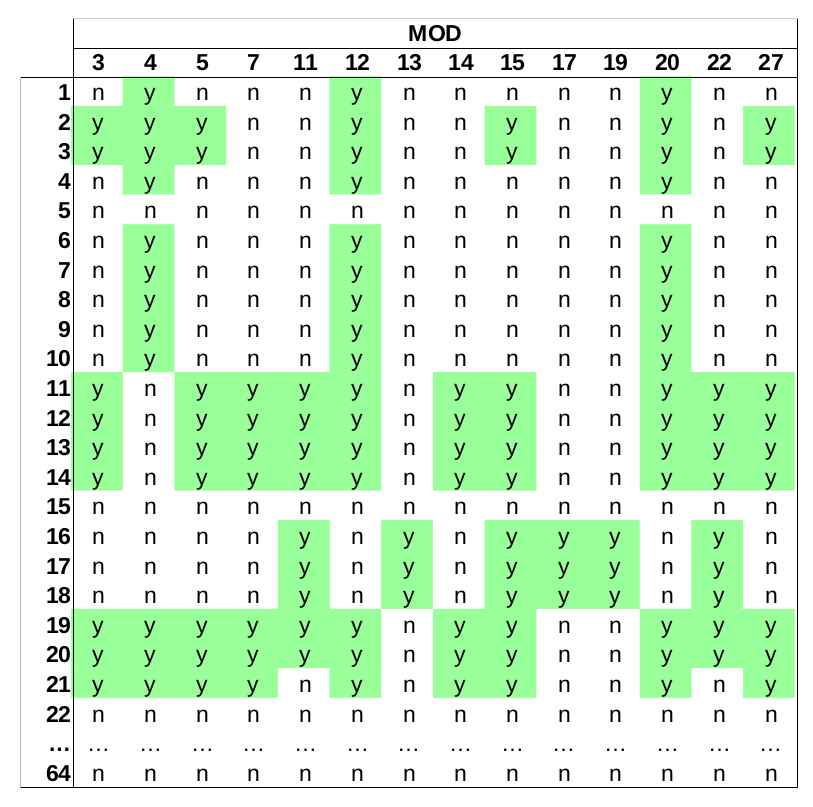
\includegraphics[width=0.96\linewidth]{../tex/images/mod_analysis}
        \end{minipage}%
        \begin{minipage}{.5\textwidth}
          \centering
          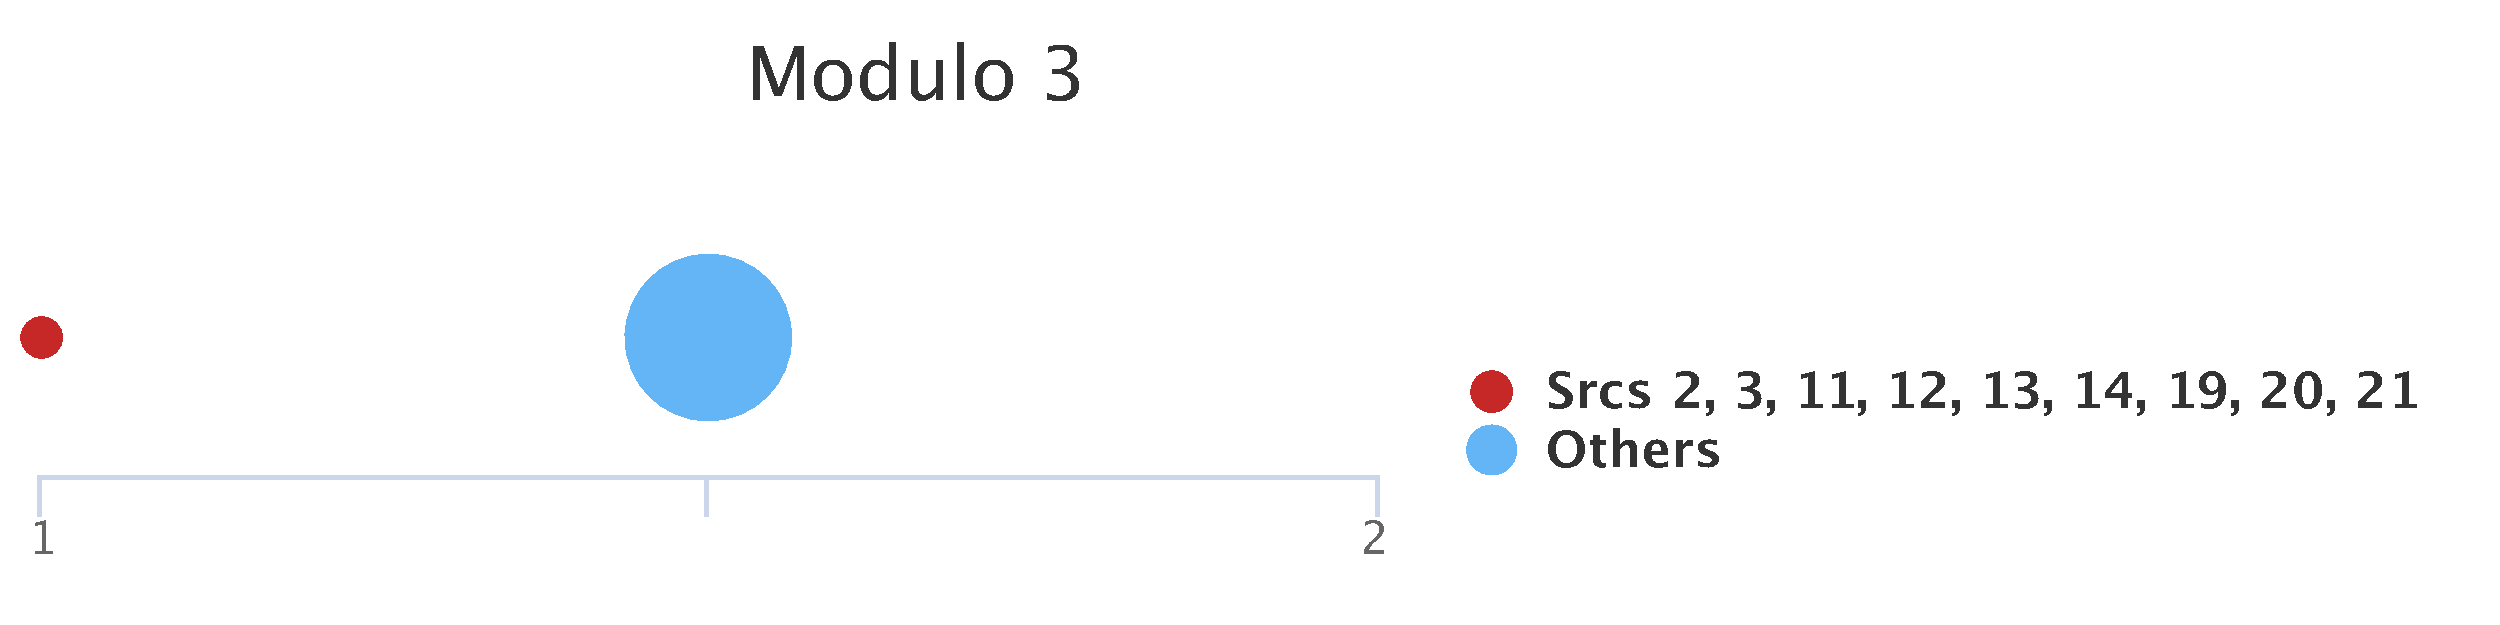
\includegraphics[width=0.96\linewidth]{../tex/images/analysis/mod3}
          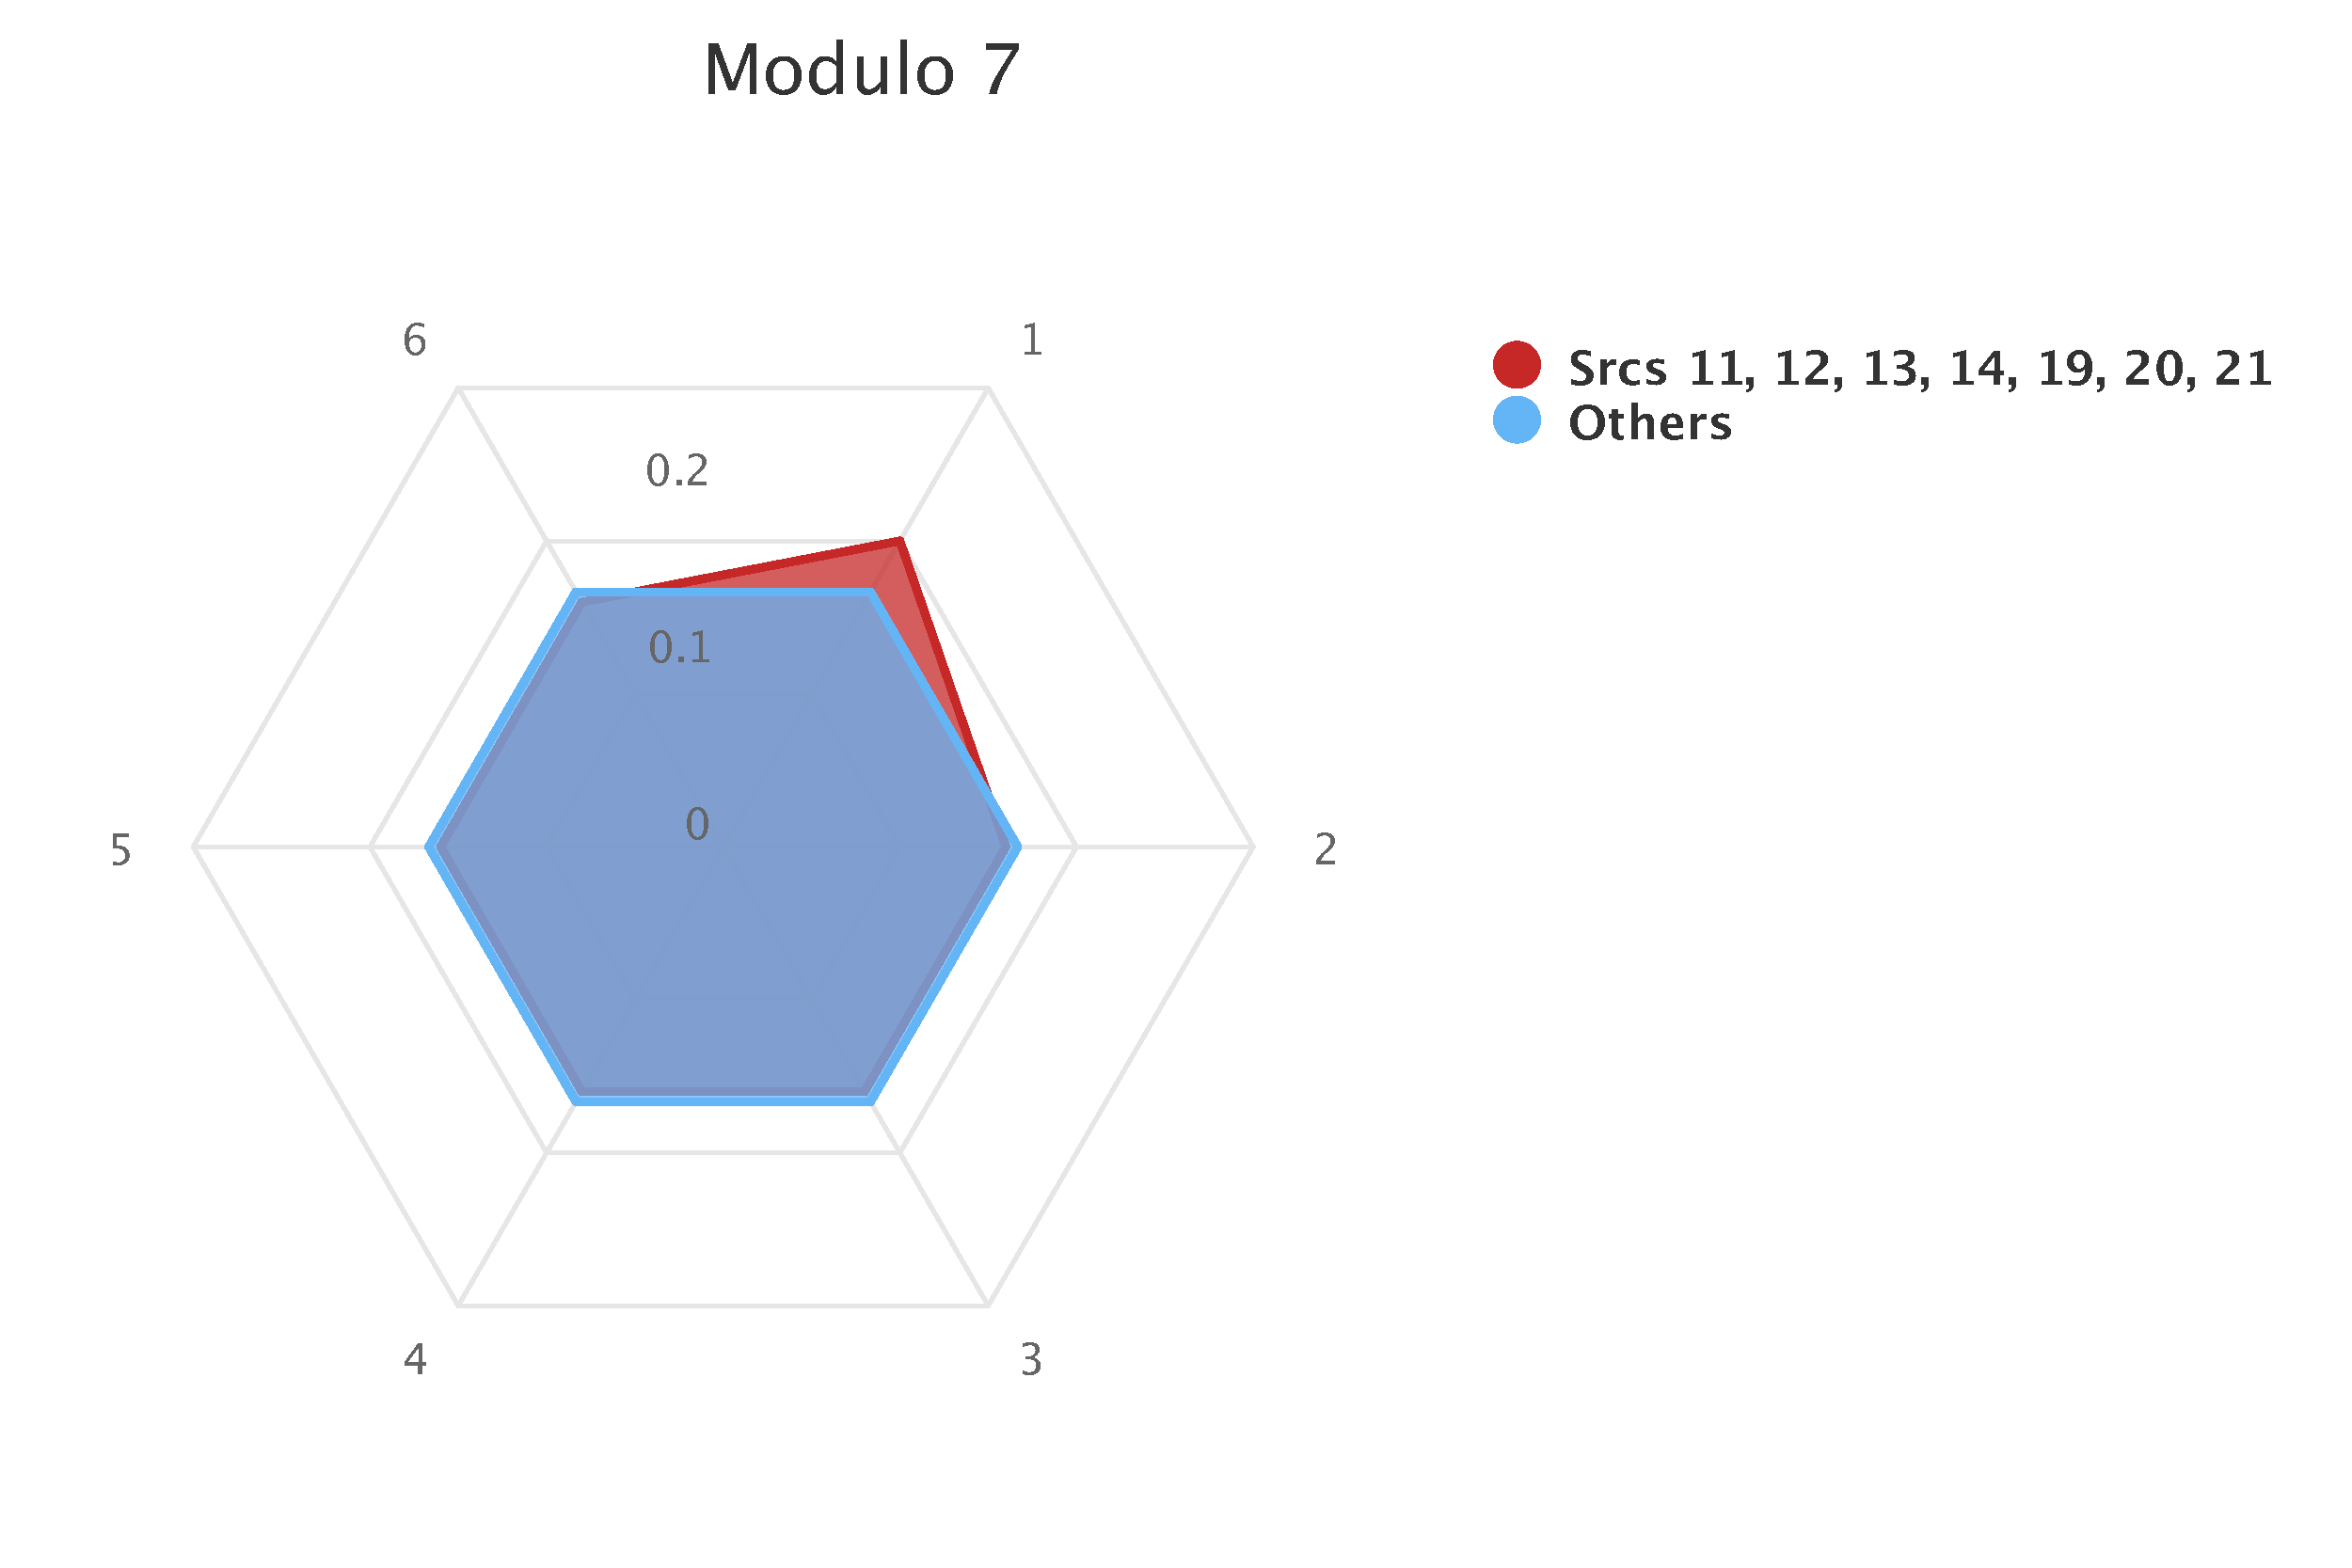
\includegraphics[width=0.96\linewidth]{../tex/images/analysis/mod7}
        \end{minipage}
      \end{figure}     
      
    \end{frame}

    \section{Implementation}
    \begin{frame}{Implementation}
      \begin{itemize}
        \Fontsmall
        \item solving binary vector to group classification problem
        \item defined flow of the application, 5 tasks defined ({\color{fibeamer@yellow}{\textbf{SCAN}}}, {\color{fibeamer@yellow}{\textbf{ANALYZE}}}, {\color{fibeamer@yellow}{\textbf{GENERATE}}}, {\color{fibeamer@yellow}{\textbf{TRAIN}}}, {\color{fibeamer@yellow}{\textbf{CLASSIFY}}})
        \item all tasks accessible via CLI, also possible on Metacentrum
        \item focus on parallel run and extensibility        
      \end{itemize}
      \begin{figure}[H]
        \centering
        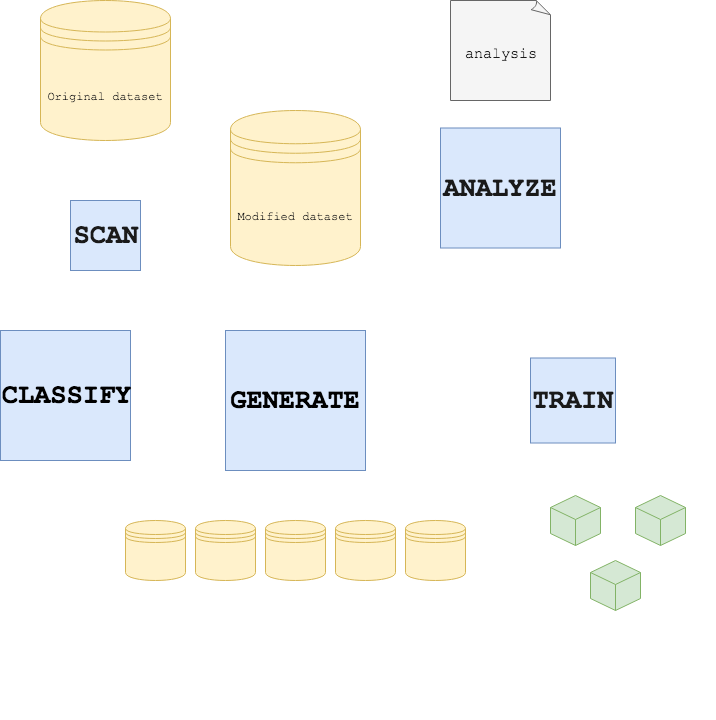
\includegraphics[width=0.5\linewidth]{../tex/images/thesis_model_img}
      \end{figure}     
    \end{frame}

    \subsection{tasks}
    \begin{frame}{SCAN}
      \begin{itemize}
        \item original dataset had around 2000 CSV files with no specific namespace
        \item \textbf{SCAN} task designed to transform the dataset into the more compact one
        \item it assigns a specific CSV file into its group based on positive/negative keyword matching
      \end{itemize}
    \end{frame}

    \begin{frame}{ANALYZE}
      \begin{figure}[H]
        \centering
        \begin{minipage}{.5\textwidth}
          \begin{itemize}
            \item task to perform analysis on dataset
            \item user defined features
            \item huge data is yielded in chunks
            \item auxiliary \texttt{FeatureMaker} class
          \end{itemize}          
        \end{minipage}%
        \begin{minipage}{.5\textwidth}
          \centering
          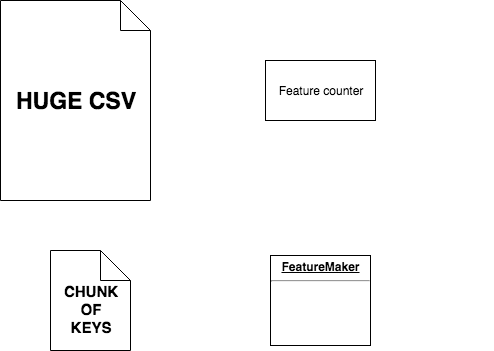
\includegraphics[width=0.98\linewidth]{../tex/images/analyze_task_img}
        \end{minipage}
      \end{figure}  
    \end{frame}

    \begin{frame}{GENERATE}
      \begin{itemize}
        \item many datasets with different properties generated
        \item used to prepare and adapt data for training
        \item functionality to:
        \begin{enumerate}
          \item generate arbitrary CSV files
          \item shuffle target file
          \item relabel and merge groups
          \item skip any source of group
          \item arbitrary number of keys per group
          \item arbitrary number of keys per line
          \item multiply training data
        \end{enumerate}
      \end{itemize}
    \end{frame}

    \begin{frame}{TRAIN}
      \begin{itemize}
        \item train and evaluate models
        \item two components \texttt{Loader} and \texttt{Model}
        \item \texttt{Loader} is reponsible for fetching data to model (optimized to work with large datasets)
        \item \texttt{Model} used via common interface (easily extensible for new models)
        \item implemented \texttt{KerasClassifier} and \texttt{SciKitClassifier}
      \end{itemize}
    \end{frame}

    \begin{frame}{CLASSIFY}
      \begin{itemize}
        \item evaluation of already trained models
        \item assigning labels to unknown keys
        \item the most important task for the end users
      \end{itemize}
    \end{frame}

    \section{Results}
    \subsection{Traditional classifiers}
    \begin{frame}{Results - traditional classifiers}
      \Fontsmall
      \begin{table}[!b]
        {\carlitoTLF % Use monospaced lining figures
        \begin{tabularx}{\textwidth}{XX}
          \toprule
          Classifier & $\sim$ accuracy \\
          \toprule 
          RadiusNeighborsClassifier & 7.50 \% \\
          QuadraticDiscriminantAnalysis & 7.68 \% \\
          ExtraTreeClassifier & 12.62 \% \\
          MLPClassifier & 12.65 \% \\
          DecisionTreeClassifier & 12.71 \% \\
          KNeighborsClassifier & 16.92 \% \\
          SGDClassifier & 20.70 \% \\
          PassiveAggressiveClassifier & 21.72 \% \\
          AdaBoostClassifier & 22.34 \% \\
          GaussianNB & 27.51 \% \\
          MultinomialNB & 28.22 \% \\
          LinearSVC & 29.93 \% \\
          LinearDiscriminantAnalysis & 30.81 \% \\
          NuSVC & 30.93 \% \\
          RidgeClassifier & 31.14 \% \\
          BernoulliNB & 31.21 \% \\
          RidgeClassifierCV & 31.22 \% \\
          SVC & 32.57 \% \\
          BaggingClassifier & 32.74 \% \\
          RandomForestClassifier & 33.04 \% \\
          ExtraTreesClassifier & 33.26 \% \\
          GradientBoostingClassifier & 33.57 \% \\ 
          \bottomrule
        \end{tabularx}}
      \end{table}
    \end{frame}
      
    \subsection{Results - neural networks}
    \begin{frame}{Results - NN model 1}
      \begin{itemize}
        \item multi layer perceptron used
        \item {\color{fibeamer@yellow}{\textbf{grid search}}} technique used for optimal topology, activation and optimizer
        \begin{itemize}
          \item sparse models performed $\sim 1 \%$  worse than denser ones
          \item the best results achieved with ReLU and leakyReLU activations
          \item optimizers did not visibly affect the overall accuracy
        \end{itemize}
        \item final model:
        \begin{itemize}
          \item input layer with the length of input vector\footnote{for 512b, the vector had length 836}
          \item hidden layer (256 neurons, ReLU)
          \item softmax layer and argmax layer on top
          \item optimizer Adam
        \end{itemize}
      \end{itemize}
    \end{frame}

    \begin{frame}{Results - NN model 1}
      \begin{figure}[H]
        \centering
        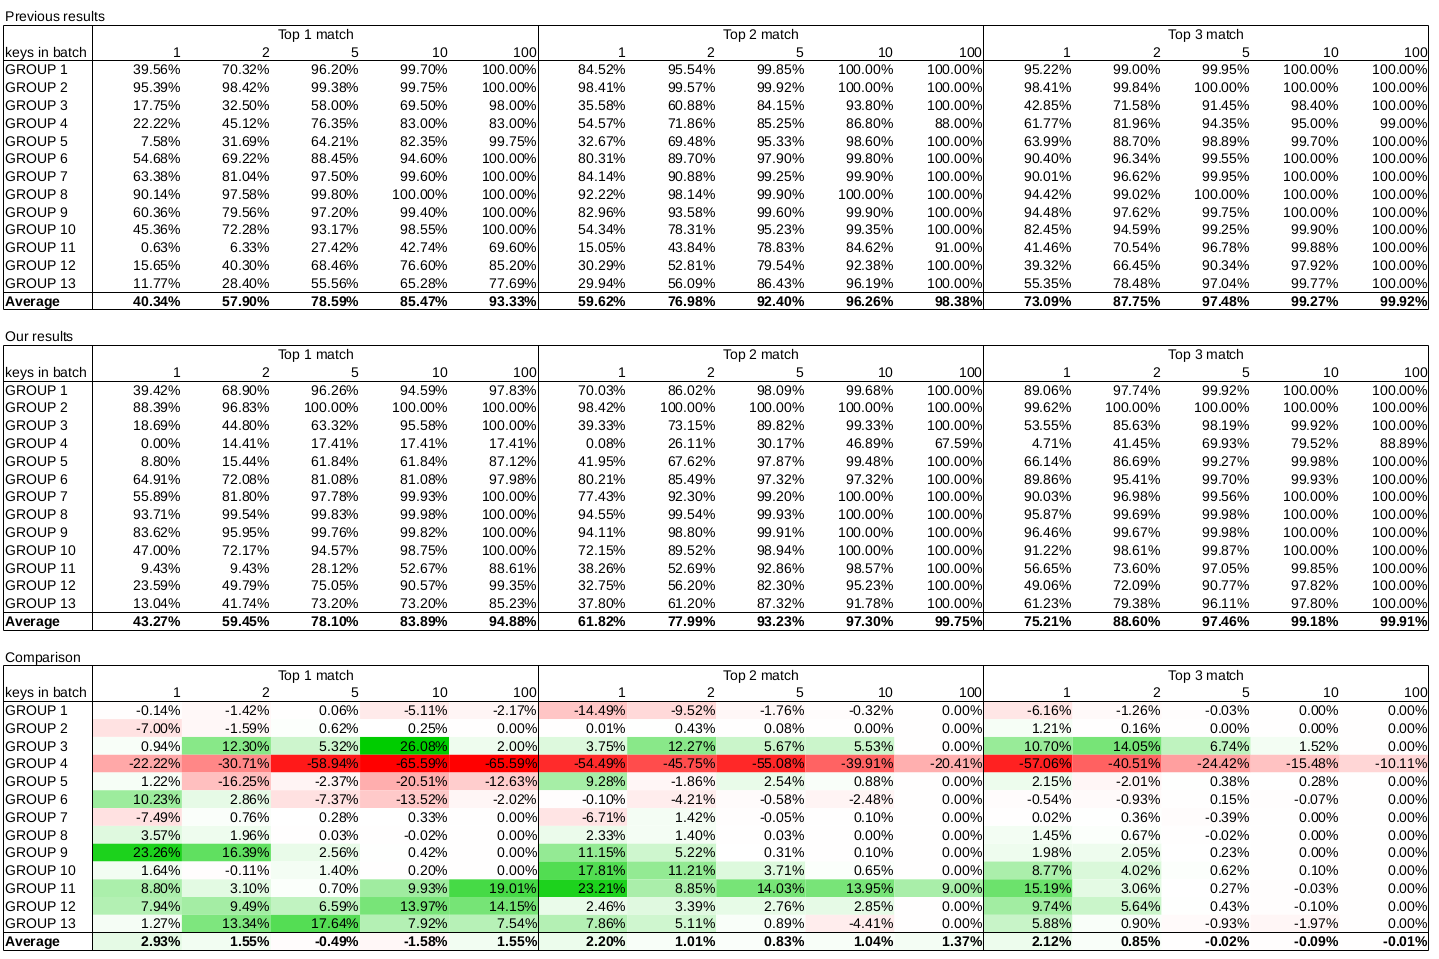
\includegraphics[width=0.98\linewidth]{../tex/images/results/comparison_13.png}
      \end{figure}  
    \end{frame}

    \begin{frame}{Results - NN model 2}
      \begin{itemize}
        \item consists of 13 binary classifiers for each group
        \item each classifier trained and evaluated individually
        \item input is fed to all of them
        \item softmax and argmax layer on top to merge results together
      \end{itemize}
      \begin{figure}[H]
        \begin{minipage}{.33\textwidth}         
          \centering
          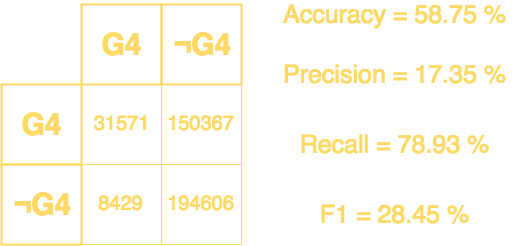
\includegraphics[width=0.95\linewidth]{../tex/images/results/rese_g4_512_img}
        \end{minipage}%
        \begin{minipage}{.33\textwidth}         
          \centering
          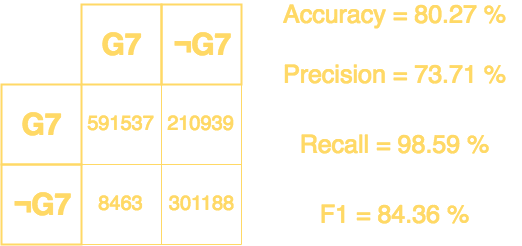
\includegraphics[width=0.95\linewidth]{../tex/images/results/rese_g7_512_img}
        \end{minipage}%
        \begin{minipage}{.33\textwidth}         
          \centering
          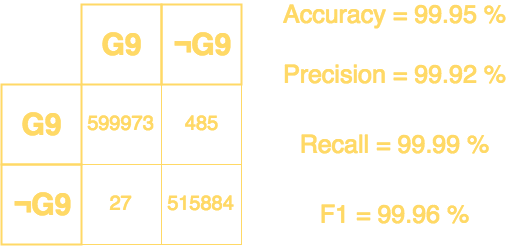
\includegraphics[width=0.95\linewidth]{../tex/images/results/rese_g9_512_img}
        \end{minipage}%        
      \end{figure}
    \end{frame}

    \begin{frame}{Results - NN model 2}
      \Fontsmall
      \begin{table}[!b]
        {\carlitoTLF % Use monospaced lining figures
        \begin{tabularx}{\textwidth}{r|X|X|X}
\toprule
          Group & Top 1 match                     & Top 2 match                     & Top 3 match                     \\
\bottomrule
1     & 45.23 \% {\color[HTML]{9B9B9B} (39.56 \%)} & 60.10 \% {\color[HTML]{9B9B9B} (84.52 \%)} & 87.87 \% {\color[HTML]{9B9B9B} (95.22 \%)} \\

2     & 70.79 \% {\color[HTML]{9B9B9B} (95.39 \%)} & 95.54 \% {\color[HTML]{9B9B9B} (98.41 \%)} & 99.29 \% {\color[HTML]{9B9B9B} (98.41 \%)} \\

3     & 18.71 \% {\color[HTML]{9B9B9B} (17.75 \%)} & 41.58 \% {\color[HTML]{9B9B9B} (35.58 \%)} & 55.79 \% {\color[HTML]{9B9B9B} (42.85 \%)} \\

4     & 34.08 \% {\color[HTML]{9B9B9B} (22.22 \%)} & 58.88 \% {\color[HTML]{9B9B9B} (54.57 \%)} & 74.88 \% {\color[HTML]{9B9B9B} (61.77 \%)} \\

5     & 8.59 \% {\color[HTML]{9B9B9B}( 7.58 \%)}  & 30.64 \% {\color[HTML]{9B9B9B} (32.67 \%)} & 58.31 \% {\color[HTML]{9B9B9B} (63.99 \%)} \\

6     & 23.44 \% {\color[HTML]{9B9B9B} (54.68 \%)} & 43.44 \% {\color[HTML]{9B9B9B} (80.31 \%)} & 55.55 \% {\color[HTML]{9B9B9B} (90.40 \%)} \\

7     & 78.14 \% {\color[HTML]{9B9B9B} (63.38 \%)} & 93.75 \% {\color[HTML]{9B9B9B} (84.14 \%)} & 96.62 \% {\color[HTML]{9B9B9B} (90.01 \%)} \\

8     & 93.53 \% {\color[HTML]{9B9B9B} (90.14 \%)} & 93.69 \% {\color[HTML]{9B9B9B} (92.22 \%)} & 94.54 \% {\color[HTML]{9B9B9B} (94.42 \%)} \\

9     & 99.77 \% {\color[HTML]{9B9B9B} (60.36 \%)} & 99.97 \% {\color[HTML]{9B9B9B} (82.96 \%)} & 99.99 \% {\color[HTML]{9B9B9B} (94.48 \%)} \\

10    & 45.61 \% {\color[HTML]{9B9B9B} (45.36 \%)} & 83.81 \% {\color[HTML]{9B9B9B} (54.34 \%)} & 94.68 \% {\color[HTML]{9B9B9B} (82.45 \%)} \\

11    & 0.94 \% {\color[HTML]{9B9B9B}( 0.63 \%)}  & 19.87 \% {\color[HTML]{9B9B9B} (15.05 \%)} & 50.01 \% {\color[HTML]{9B9B9B} (41.46 \%)} \\

12    & 24.21 \% {\color[HTML]{9B9B9B} (15.65 \%)} & 30.75 \% {\color[HTML]{9B9B9B} (30.29 \%)} & 41.90 \% {\color[HTML]{9B9B9B} (39.32 \%)} \\

13    & 21.81 \% {\color[HTML]{9B9B9B} (11.77 \%)} & 49.36 \% {\color[HTML]{9B9B9B} (29.94 \%)} & 64.19 \% {\color[HTML]{9B9B9B} (55.35 \%)} \\

\toprule
TOTAL & 41.12 \% {\color[HTML]{9B9B9B} (40.34 \%)} & 59.82 \% {\color[HTML]{9B9B9B} (59.62 \%)} & 73.36 \% {\color[HTML]{9B9B9B} (73.09 \%)} \\
\bottomrule
        \end{tabularx}}
      \end{table}
    \end{frame}

    \section{Conclusion}

    \begin{frame}{Conclusion}
      \begin{itemize}
        \item TODO
      \end{itemize}
    \end{frame}

  \end{darkframes}
\end{document}